\documentclass[12pt]{article}

%Aus dem LaTex Template der Universit�t Stuttgart
%------------------------------------------------
\usepackage[utf8]{inputenc}
\usepackage[T1]{fontenc}
\usepackage[sfdefault]{ClearSans} %% option 'sfdefault' activates Clear Sans as the default text font
\usepackage{cmap}
\usepackage[ngerman]{babel}
\usepackage{graphicx}
\usepackage[pdftex,hyperref,dvipsnames]{xcolor}
\usepackage{listings}
\usepackage[a4paper,lmargin={2cm},rmargin={2cm},tmargin={3.5cm},bmargin = {2.5cm},headheight = {4cm}]{geometry}
\usepackage{amsmath,amssymb,amstext,amsthm}
\usepackage[lined,algonl,boxed]{algorithm2e}
\usepackage{tikz}
\usepackage{hyperref}
\usepackage{url}
\usepackage[inline]{enumitem} % Erm�glicht �ndern der enum Item Zahlen
\usepackage[headsepline]{scrpage2} 
\usepackage{algorithmic} % F�r Pseudocode
\usepackage{ marvosym } % f�r Pfeil(e)
\usepackage{booktabs} % F�r die sch�neren Booktabs-Tabellen
\usepackage{tikz}
\usepackage{pdfpages}
\usepackage{blindtext}
\usepackage{scrextend}
\usepackage{pdfpages}
\usepackage{natbib} % Yannis hat das importiert; TODO: nachfragen, zu was das gut ist
\pagestyle{scrheadings} 
\usetikzlibrary{automata,positioning}

\begin{document}
	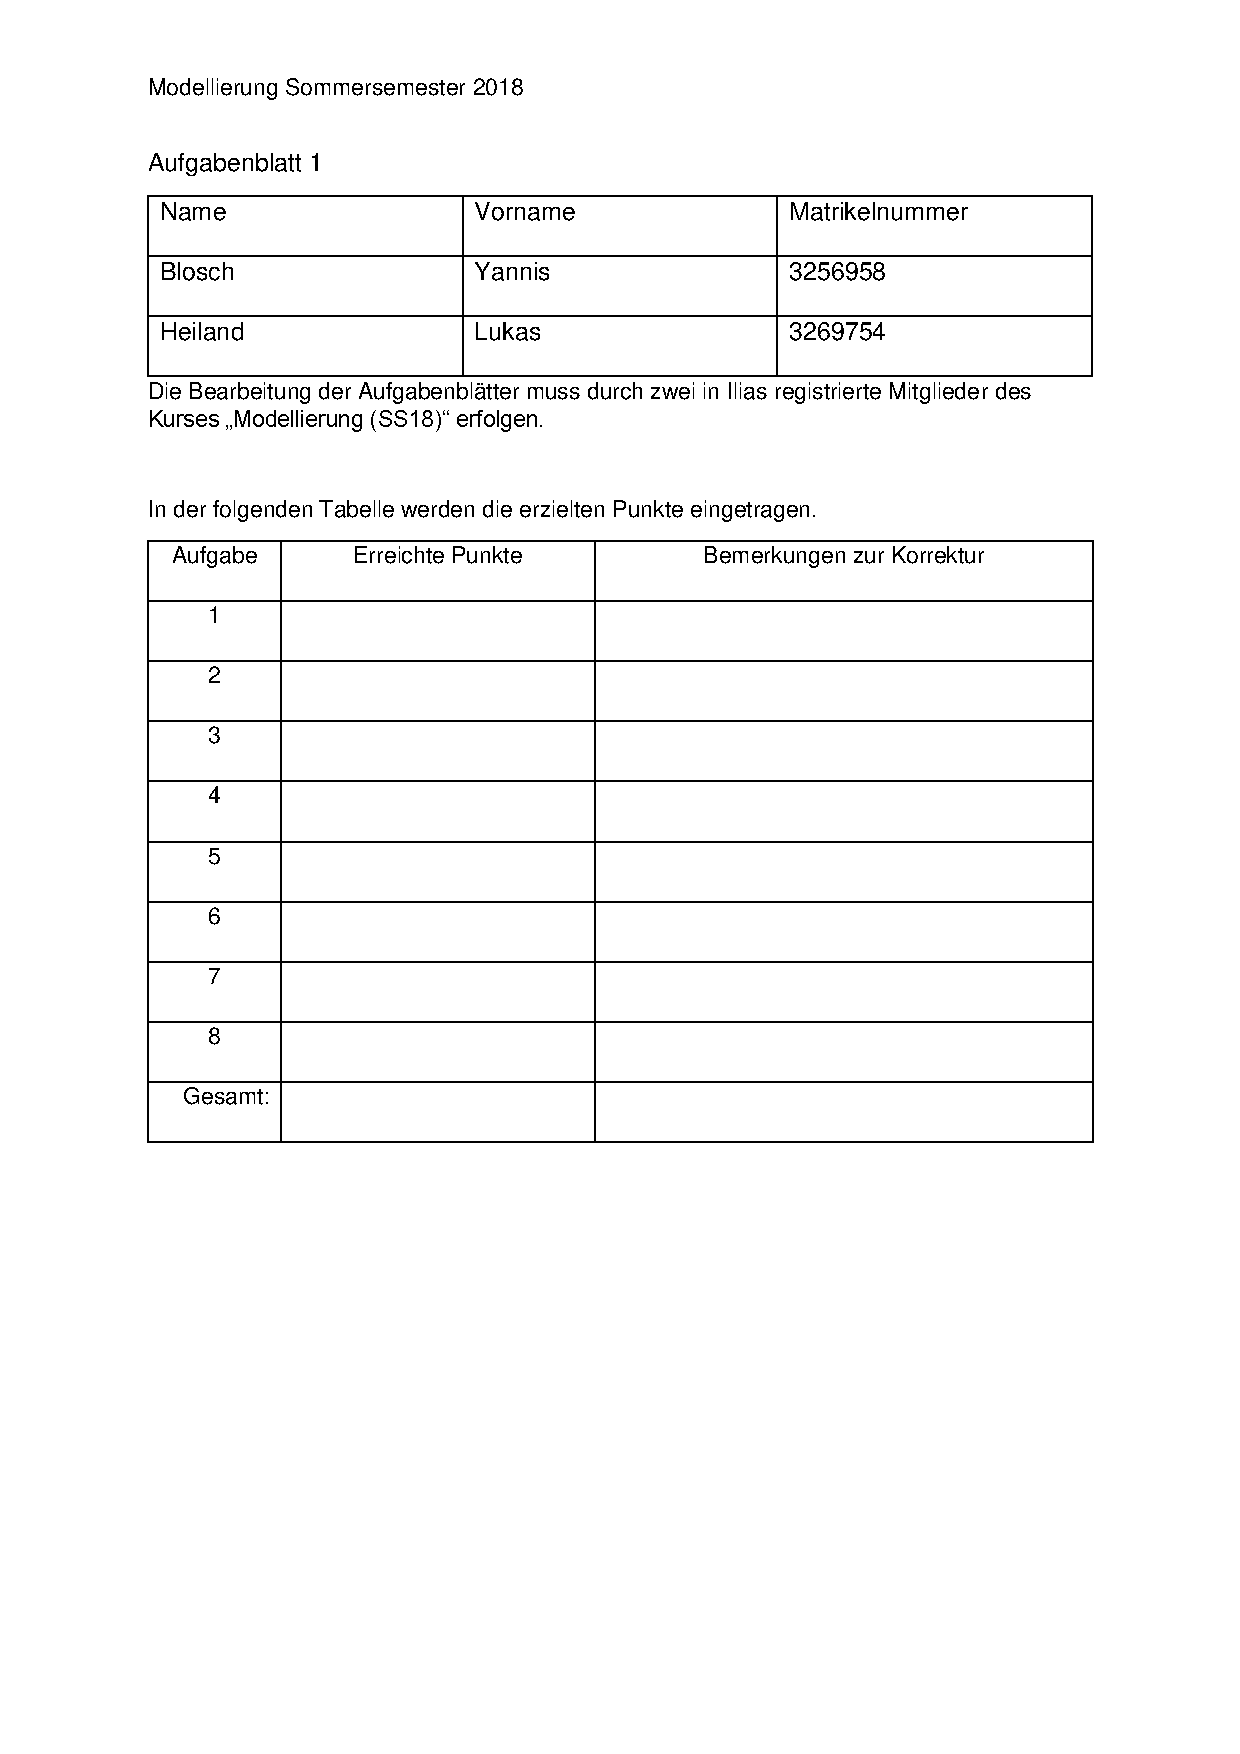
\includepdf[pages=-]{deckblatt.pdf}
	
	% Counter für das Blatt und die Aufgabennummer.
% Ersetze die Nummer des Übungsblattes und die Nummer der Aufgabe
% den Anforderungen entsprechend.
% Beachte:
% \setcounter{countername}{number}: Legt den Wert des Counters fest
% \stepcounter{countername}: Erhöht den Wert des Counters um 1.
\newcounter{sheetnr}
\setcounter{sheetnr}{1} % Nummer des Übungsblattes
\newcounter{exnum}
\setcounter{exnum}{1} % Nummer der Aufgabe

% Befehl für die Aufgabentitel
\newcommand{\exercise}[1]{\section*{Aufgabe \theexnum\stepcounter{exnum} #1}} % Befehl für Aufgabentitel

% Formatierung der Kopfzeile
% \ohead: Setzt rechten Teil der Kopfzeile mit
% Namen und Matrikelnummern aller Bearbeiter
\ohead{Yannis Blosch (3256958)\\
Lukas Heiland (3269754)}
% \chead{} kann mittleren Kopfzeilen Teil sezten
% \ihead: Setzt linken Teil der Kopfzeile mit
% Modulnamen, Semester und Übungsblattnummer
\ihead{Modellierung\\
Sommersemester 2018\\
Blatt \thesheetnr}
	
	\section*{Aufgabe 2.1}
	%Quelle(https://andydunkel.net/assets/wp-custom/docs/datenbanken.pdf)
	
	
	
		
		%a)
		%Geben Sie zunächst die Relationen mit ihren Attributen in folgender Notation an: 

		%Relation ( Attribut1, Attribut2, …, Attributn) 
		%Verwenden Sie Namen von Relationen und Attributen, die möglichst nahe an den Vorgaben im ER-Diagramm sind. Erzeugen Sie keine überflüssigen Relationen oder Attribute! Markieren Sie die Primärschlüssel der Relationen durch Unterstreichung. Verwenden Sie zur Umsetzung der is-aBeziehung das Hausklassenmodell. 
		\paragraph*{a.}
			Bahnhof (\underline{Ort}, \underline{Haltestelle},Kategorie)\\[1.3em]
			
			Fahrkarte (\underline{FahrkartenNr}, Reisedatum, Startzeit, Pl"atze)\\[1.3em]
			
			Linie (\underline{Bezeichnung}, Betreiber)\\[1.3em]
			
			Zug (\underline{ZugNr}, Eigentümer)\\[1.3em]
			
			Person (\underline{Name}, \underline{Geburtsdatum}, Adresse) \\[1,3em]
			
			Bahnkundin (\underline{Name}, \underline{Geburtsdatum}, Adresse, KundenNr)\\[1,3em]
			
			Mitarbeiter (\underline{Name}, \underline{Geburtsdatum},  Adresse, Gehalt)\\[1,3em]
		
		%b)
		%Geben Sie alle Fremdschlüsselattribute an und benennen Sie die Relationen und Attribute, auf die diese jeweils verweisen in der folgenden Notation: 
		
		%Relation1(Attribut1) -> Relation2(Attribut2) 	
		\paragraph*{b.}	
			
			Zug (\underline{ZugNr}, Eigentümer)\\[1.3em]
			
			Wagen (\underline{WagenNr}, \underline{ZugNr} REFERENCES Zug, Plätze)\\[1.3em]
			
		%c)
		% Geben Sie für die Umsetzung der is-a-Beziehung eine Lösung im Partitionierungsmodell an. Geben Sie alle Relationen an, die im Zusammenhang mit der is-a-Beziehung erforderlich sind. Erläutern Sie, wie sich die zugehörigen Relationen und deren Attribute im Vergleich zum Hausklassenmodell ändern? 
		\paragraph*{c.}
			Person (\underline{Name}, \underline{Geburtsdatum}, Adresse) \\[1,3em]
			
			Bahnkundin (\underline{Name}, \underline{Geburtsdatum}, KundenNr) \\[1,3em]
			
			Mitarbeiter (\underline{Name}, \underline{Geburtsdatum}, Gehalt) \\[1,3em]
		
			Nur neu hinzukommende Attribute und Primärschlüssel werden mit in die Relation aufgenommen.
	
	\newpage	
	\section*{Aufgabe 2.2}
	
		\paragraph*{a)}
			$\pi_{Name, Sitz}(\sigma_{TeilNr=25}(Teil)(Lieferant))$
	
		
\end{document}